\chapter{Interpretation of Search Results Within Theoretical Models}
\section{Introduction}
It is very often the case that a search for \ac{NP} will yield results
consistent with the currently accepted theory (which, in most particle physics
contexts would be the \ac{SM}). In the absence of a discovery\footnote{Certain
  models may also have a role to play in the characterisation of a discovery.},
it is often desirable to provide additional information in the form of a
statistical interpretation of the results. Such an interpretation typically
serves the following goals:
\begin{itemize}
\item Indicate the strength of the analysis in searching for the proposed model
  or set of models. This can then be used as an objective measure by which to
  rank different analyses or to benchmark the progress of a single analysis as
  data is collected.
\item Falsify, to some confidence level, a particular theory or some region of
  parameter space within that theory. In the case of a reasonably generic model,
  parameterised in such a way that it may represent other theories (or
  approximate their experimental signature), theorists may be able to
  test the predictions of a variety of models directly against the results of
  the interpretation. This will be discussed further in Section~\ref{sec:sms}.
\item Guide the optimisation of analysis cuts and object selection.
\end{itemize}

Providing an interpretation invariably necessitates some choice of theory or
phenomenological model against which to test the results. The range of theories
will of course depend strongly on the inclusiveness of the experiment. Indeed,
in many cases a single theory will have motivated the analysis in the first
place and the choice of model will be clear. In other cases, the analysis have
been designed to be as inclusive as possible and therefore sensitive to an array
of theories. Typically this is achieved by focussing on a particular detector
signature (for instance missing transverse energy), where a deviation from the
\ac{SM} is a common feature of many \ac{NP} scenarios. Another similar issue
arises when the model being tested is not well defined with a large number of
free parameters which affect the experimental expectations.

\ac{SUSY} searches in particular are subject to these
considerationss. Firstly, as discussed in Section~\ref{sec:susy}, the theory
has a large number of free parameters which may drastically change the
experimental signature. Secondly, whilst a \ac{SUSY} specific interpretation is
possible in principal, it is in some sense not the best use of the experimental
data. The large, multi-dimensional \ac{SUSY} parameter space and corresponding
variation in the physics signatures necessitates an inclusive analysis
strategy - typically looking for high jet multiplicities in association with
large missing transverse energy. Such signatures may occur in a variety of
potential \ac{NP} theories. With an appropriate interpretation, the results of
an inclusive \ac{SUSY} search can be used to draw conclusions about these
theories, restricting their parameter space or ruling them out altogether.

\ac{SUSY} searches at the \ac{LHC} have typically provided two
interpretations. The first, within a very restricted class of \ac{SUSY} theories
known as the \ac{CMSSM}. The second, within one or more so-called ``Simplified
Models'', chosen by theorists to represent a wide range of possible \ac{NP}
theories, categorised according to their phenomenological properties.

\section{Models}
\subsection{\acl{CMSSM}}

\subsection{Simplified Models}
\label{sec:sms}
It is often the case that theorists, having devised some theory, and made
concrete phenomenological predictions from it, wish to test it against
experimental data. The difficulty then arises of taking these predictions and
translating them into a form where they can be compared directly with
experimental results. Typically, these results will be provided in the form of
one or more event yields, corresponding background predictions and statistical
and systematic uncertainties. In some (but probably not most) cases, the
relevant correlations will also be included. The theorist must then take the
predictions of the theory and apply experimental resolution effects to them in
order to simulate the expected signal yield. Modern detectors are highly complex
and require very complex simulation to precisely model all of the resolution
and acceptance effects. In some cases, in particular for relatively simple
kinematic quantities, a simplified parameterisation may suffice but detailed
checks will be required to confirm that a given approximation reproduces, with
adequate fidelity the full detector simulation or the actual recorded data. If
it can be confirmed that this is the case, the theorist may then proceed to redo
the work of the experimentalist in modelling the various statistical and
systematic effects in the form of a likelihood function. Finally, they may then
utilise all of these components to produce their own statistical interpretation
of the data against the chosen theory.

Clearly, this procedure is both laborious and error-prone. It was therefore
proposed that the \ac{LHC} experiments would provide a richer interpretation in
the context of a set of ``Simplified Models''. Broadly speaking, a simplified
model is a highly simplifed effective theory, chosen to characterise a
particular phenomological scenario present within one or more \ac{NP}
models. Free parameters which have little effect on the physics are integrated
out, leaving only those with a large effect on the physics. In constructing a
number of these models, the full space of possibly physical signatures arising
in much more complicated theories may be spanned.

Although the concept of a simplified model is quite general, the discussion here
will focus on those inspired by \ac{SUSY} or ``\ac{SUSY}-like'' theories, and
more specifically those relevant to the single-leptonic experimental search
described in previous chapters.

% \todo[size=\tiny, linespacing=0.5]{Mention that SMS are used for characterisation of discovery as well as
%   design of searches}

\subsubsection{Dark Matter Models}
As discussed in Chapter~\ref{sec:susy}, a highly desirable prediction of certain
supersymmetric theories is the existence of a stable, weakly-interacting
particle or \ac{WIMP}. This is a dark matter candidate with a striking
experimental signature at collider experiments - a large missing energy
component in the transverse plane. At hadron colliders, the initally produced
particles are likely to be coloured (either squarks or gluinos) which will then
decay to the \ac{WIMP} producing a large number of jets. Together, these might
be considered the characteristics of a ``canonical'' \ac{SUSY} event at the
\ac{LHC}. Whilst the range of simplified models includes a much more generic set
of signatures, for the purposes of this discussion we will choose two topologies
which exhibit these characteristics.

Both topologies emulate certain aspects of \ac{SUSY} phenomenology albet in a
simpler framework with greater generality. In order to distinguish the particle
content from pure \ac{SUSY} theories, a different notation will be used. The
first topology, T1 arises from pair production of neutral, coloured objects
$\tilde{G}$ (the gluinos of \ac{SUSY} theories). The second topology, T2 instead
arises from pair production of a charged, coloured particle $\tilde{Q}$
(effectively the squark). Both topologies consider only pair-produced
superpartners or in other words they conserve an $R$-parity type quantum
number. In addition to the superpartners produced in the intial interaction,
there are a number of intermediate states $\tilde{X}^0_i$ and
$\tilde{X}^{\pm}_j$. In terms of \ac{SUSY} particles these would be analogues of
the neutralinos and charginos respectively. Importantly, $\tilde{X}^0_1$ is defined to
be the lightest superpartner - a dark matter candidate and the source of missing
energy in the events.

\subsubsection{T1 Simplified Model Topology}
In the T1 simplified model, the $\tilde{Q}$ are assumed to be heavier than the
$\tilde{G}$ and thus the only decay mode available is via an off-shell
$\tilde{Q}$. Three such cascade decays leading to the $\tilde{X}^0_1$ are shown in
Figure~\ref{fig:gluino_sms_decays}. The first, is a direct 3-body decay to the
\ac{LSP}. This dominates in the following \ac{mSUGRA} scenarios:
\begin{itemize}
\item $\PSgxzi \approx \PSB$ and the $\PSq_{R}$ are lightest or the $\PSW$ is kinematically
  inaccessible.
\item $\PSgxzi \approx \PSW$ and either $\PSq_{L}$ are lightest or there is no
  splitting between the left and right-handed squarks.
\item $\PSgxzi \approx \PSH$ and either heavy-flavour squarks are inaccessible or
  $\PSB$ and $PSW$ are inaccessible.
\end{itemize}

\begin{figure}
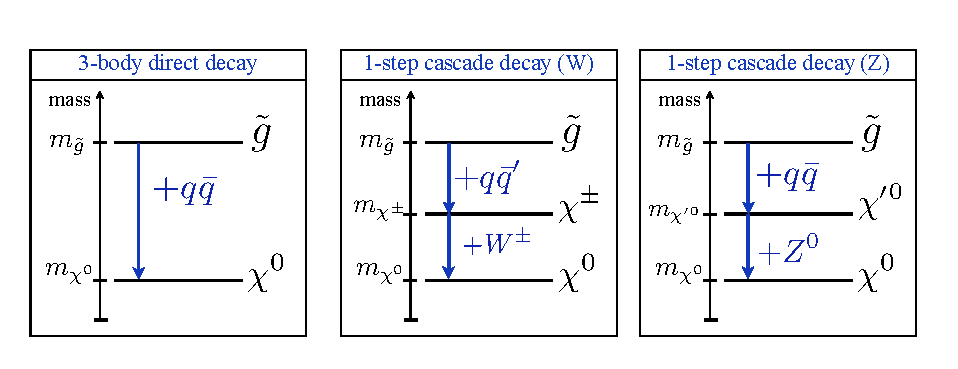
\includegraphics[width=\textwidth]{fig/gluino_sms_decays}
\caption{Illustration of the gluino decay modes within the T1 simplified model
  topology. \cite{alves_simplified_2011}}
\label{fig:gluino_sms_decays}
\end{figure}

In most \ac{mSUGRA} or \ac{GMSB} models, the $\PSgxzi \approx \PSB$ and there is
not a strong left-right mass splitting in the squarks. Therefore, it is unlikely
for the direct decays to dominate. In most cases, 1-step cascade decays
will be favoured. In these the, gluino decays first to either a $\PSgxpm$ or a
heavy $\PSgxz$. This will subsequently decay via either a $\PW$ or a $\PZ$ to
the $\PSgxzi$.

\subsubsection{T2 Simplified Model Topology}
For the T2 simplified model, the produced $\tilde{Q}$ can decay as follows:
\begin{eqnarray}
\tilde{Q} &\longrightarrow \tilde{G} \Pq \label{eqn:t2gluino}\\
\tilde{Q} &\longrightarrow \tilde{X}^0_i \Pq \\
\tilde{Q} &\longrightarrow \tilde{X}^\pm_i \Pq
\end{eqnarray}
If allowed, the \ref{eqn:t2gluino} decay will dominate since it has QCD
strength.

\subsubsection{Combining Topologies}
For phenomenological purposes, each separate decay topology may be considered as
an independent simplified model. The predictions of a whole set of topologies
can then be combined by taking linear combinations. For direct comparison
against experimental data, it is desirable to simulate a desired set of
topologies within a monte-carlo generator by ``turning on'' the chosen physics
subprocesses. The model parameter space can be sampled by moving through a
lattice of values in the desired range. At each lattice site, a statistically
sufficient number of events is generated with the appropriate parameter values
inserted into the configuration of the \ac{MC} generator.

\section{Statistical Methods}
\subsection{Background}

\subsection{Modelling the Single Lepton Analysis}
As described in the previous section, the core component of many statistical
interpretations is the construction of an appopriate likelihood function. The
likelihood must model all statistical and systematic effects and is thus highly
dependent on the experiment. The situation is considerably complicated when
shape information is included, for which relevant bin-to-bin correlations must
be included.

\subsubsection{Notation}
It will be helpful to define some notation. In the following, a subscript index
is assumed to run over the binned variable in the analysis
(i.e. \STlep). All nuisance parameters are written as $\nu^{(i)}$ where the
superscript index is taken to run over some set of systematics
(e.g. $\nu^{\textrm{jes}}$ might represent a jet energy scale
uncertainty). Certain variables $x$ are known to have a functional dependence on a
given nuisance parameter and are written $x(\nu)$. The nominal value of this
variable, being that which is measured in \ac{MC} or in real data is denoted
$\bar{x}$.

\subsubsection{The Likelihood Function}
In constructing the likelihood, we start by writing down the number of events
expected for each bin (assigned the index $i=0,1,2...$):
\begin{equation}
\NExpi = \NSigi(\mu, \nu^{(j)}) +
\NBkgi(\nu^{(k)}) \\
\end{equation}
where \NSigi is the expected signal yield for a chosen
signal model and \NBkgi is the data-driven background
prediction. As can be seen, the signal yield is a function of the \ac{poi} (the
signal strength) and some number of nuisance parameters where the index $j$
will run over a set of systematics relevant to the signal yield. Ignoring
signal contamination effects (which will be discussed later), the bacground
yield depends only on the nuisance parameters $\nu^{(k)}$ where $k$ is taken to run
over the set of systematics relevant to the bacground prediction.

Without giving an explicit functional form for the signal yield and background
prediction, the form of the likelihood function may be constructed. The
likelihood must include:
\begin{enumerate}
\item Statistical terms representing the likelihood of observing the given
  number of events given a certain expectation for the signal and background
  yields.
\item Terms providing prior constraints on the various nuisance
  parameters. Certain uncertainties are statistical in nature and thus,
  indepdent nuisance parameters are assigned per bin along with a corresponding
  prior pdf. In other cases, the underlying systematic variation is considered
  to have a 100\% correlated effect across the bins. In these cases, a single
  nuisance parameter and prior pdf is assigned.
\end{enumerate}

The form of the likelihood is as follows,
\begin{equation}
\mathcal{L} = \prod_i \mathcal{P}(\NExpi ; \NObsi)
\prod_{\alpha \in \Theta}  X_\alpha(\nu^{(\alpha)})
\end{equation}
where
\begin{itemize}
\item $\mathcal{P}(\mu;x)$ denotes a Poisson distribution with mean $\mu$ and value
$x$
\item The $X_\alpha(\nu^{(\alpha)})$ represent some prior pdf associated with
  each systematic $\alpha$.
\end{itemize}

\subsubsection{The Signal Yield}
The signal yield per bin is constructed as follows
\begin{equation}
\NSigi = \mu \times \epsilon_i(\nu^{(\alpha)}) \times \sigma \times L \times \nu^{\textrm{lumi}}
\end{equation}

with
\begin{itemize}
\item $\epsilon_i(\nu^{(\alpha)})$ is the efficiency of the $i$th bin assumed to be
  dependent on a set of nuisance parameters $\nu^{(\alpha)}$.
\item $\sigma$ the cross-section of the signal model being considered,
\item $L$ the integrated luminosity,
\item $\nu^{\textrm{lumi}}$ the nuisance parameter associated with uncertainty in the
estimate of the integrated luminosity.
\end{itemize}

\subsubsection{Background Prediction}
The background prediction per bin is then written as
\begin{equation}
\NBkgi = \RCSi(\nu_i^{(\alpha)}, \nu^{(\beta)}) \times \NControli(\nu_i^{(\gamma)})
\end{equation}
where
\begin{itemize}
\item \RCSi is the translation ratio as defined in Section TODO,
\item The nuisance parameters $\nu_i^{(\alpha)}$ and $\nu_i^{\gamma}$ represent
  statistical uncertainties uncorrelated between the bins.
\item The nuisance parameters $\nu_i^{(\beta)}$ represent systematic
  uncertainties assumed to be 100\% correlated across the bins.
\item \NControli the observed number of events in the control region
($L_P > 0.3$)
\end{itemize}

\subsubsection{Parameterising Systematics}
In reality, it is almost always impossible to obtain a full functional form for
a variable $x$ (e.g. \RCSi, \NControli) in terms of a set of nuisance parameters
$\nu^{(\alpha)}$. Writing the Taylor expansion of $x(\nu^{(\alpha)})$ for two terms to
second order,
\begin{align*}
 x(\nu^{(A)}, \nu^{(B)})\bigg|_{\substack{\nu^{(A)} = a\\ \nu^{(B)} = b}} \approx
x(a,b) +
(\nu^{(A)} - a)\left.\frac{\partial x}{\partial\nu^{(A)}}\right|_{\nu^{(A)}=a} +
(\nu^{(B)} - b)\left.\frac{\partial x}{\partial\nu^{(B)}}\right|_{\nu^{(B)}=b} +\\
\frac{1}{2!}\left[
(\nu^{(A)} - a)^2 \frac{\partial^2 x}{\partial \left(\nu^{(A)}\right)^2}
+ (\nu^{(B)} - b)^2 \frac{\partial^2 x}{\partial \left(\nu^{(B)}\right)^2}
+ 2(\nu^{(A)} - a)(\nu^{(B)} - b)\frac{\partial^2 x}{\partial
  \nu^{(A)}\partial\nu^{(B)}}
\right]
\end{align*}
Assuming the expansion is performed with respect to the mean of x, $\bar{x}$,
the values of $a$ and $b$ are seen to be the mean values of the corresponding nuisance
parameters. For small deviations from the mean,
\begin{equation}
 (\nu^{(A)} - a) \sim (\nu^{(B)} - b) \sim \epsilon \sim 0
\end{equation}
and ignoring terms $O(\epsilon^2)$

\begin{equation}
x(\nu^{(A)}, \nu^{(B)}) \approx \bar{x} +
(\nu^{(A)} - a)\left.\frac{\partial x}{\partial\nu^{(A)}}\right|_{\nu^{(A)}=a} +
(\nu^{(B)} - b)\left.\frac{\partial x}{\partial\nu^{(B)}}\right|_{\nu^{(B)}=b}
\label{eqn:stats:taylor}
\end{equation}
Since the derivatives in Equation~\ref{eqn:stats:taylor} will in practice be
derived from some finite variation of the underlying quantity associated with
each nuisance parameter, the infinitessimal derivatives must be replaced by
finite changes. It is also sensible to set $a=b=0$.
\begin{equation}
x(\nu^{(A)}, \nu^{(B)}) \approx \bar{x} +
\nu^{(A)}\frac{\Delta x}{\Delta\nu^{(A)}} +
\nu^{(B)}\frac{\Delta x}{\Delta\nu^{(B)}}
\label{eqn:stats:taylor2}
\end{equation}
Since the value of $x$ is often associated with a physical quantity such as an
efficiency or an event yield, it is desirable to constrain it to positive
values. This can be achieved providing the range of each nuisance parameter is
set such that
\begin{equation}
\nu^{j}\times\frac{\Delta x}{\Delta \nu^{(\alpha)}} < \bar{x}
\end{equation}

The previous derivation can be simply extended two $N > 2$ nuisance
parameters. Generalising and rewriting Equation~\ref{eqn:stats:taylor2},
\begin{eqnarray*}
x(\nu^{(A)}, \nu^{(B)}, \ldots) &\approx& \bar{x} +
\nu^{(A)}\frac{\Delta x}{\Delta\nu^{(A)}} +
\nu^{(B)}\frac{\Delta x}{\Delta\nu^{(B)}} + \ldots \\
&\approx& \frac{1}{\bar{x}^{N-1}} \left\{ \bar{x}^N +
\bar{x}^{N-1} \nu^{(A)}\frac{\Delta x}{\Delta\nu^{(A)}} +
\bar{x}^{N-1} \nu^{(B)}\frac{\Delta x}{\Delta\nu^{(B)}} + \ldots \right\}
\end{eqnarray*}
Trying to rewrite as a product,
\begin{eqnarray*}
\prod_{j=A, B, \ldots} \left(\bar{x} + \frac{\Delta x}{\Delta\nu^{(\alpha)}}\right) &=&
\bar{x}^N + \bar{x}^{N-1} \sum_{j=A, B, \ldots} \nu^{(\alpha)}\frac{\Delta x}{\Delta \nu^{(\alpha)}} \\
&&+ \bar{x}^{N-2}\sum_{j=A, B, \ldots} \sum_{k=A, B, \ldots} \nu^{(\alpha)}\nu^{(\beta)}\frac{\Delta x}{\Delta
  \nu^{(\alpha)}}\frac{\Delta x}{\Delta \nu^{(\beta)}} \\
&&+ \ldots +O(\nu^N)
\end{eqnarray*}
Ignoring terms greater than $O(\nu^2)$,
\begin{eqnarray*}
\prod_{j=A, B, \ldots} \left(\bar{x} + \frac{\Delta x}{\Delta\nu^{(\alpha)}}\right) &\approx&
\bar{x}^N + \bar{x}^{N-1} \sum_{j=A, B, \ldots} \nu^{(\alpha)}\frac{\Delta x}{\Delta
  \nu^{(\alpha)}} \\
&\approx& \bar{x}^{N-1} x(\nu^{(A)}, \nu^{(B)}, \ldots)
\end{eqnarray*}
and therefore
\begin{equation}
x(\nu^{(A)}, \nu^{(B)}, \ldots) \approx \frac{1}{\bar{x}^{N-1}} \prod_{j = A, B,
  \ldots} \left(\bar{x} + \frac{\Delta x}{\Delta\nu^{(\alpha)}}\right) \approx
\bar{x} \prod_{j = A, B,
  \ldots} \frac{1}{\bar{x}}\left(\bar{x} + \frac{\Delta x}{\Delta\nu^{(\alpha)}}\right)
\label{eqn:stats:systderiv}
\end{equation}

Using Equation~\ref{eqn:stats:systderiv}, the signal yield can be rewritten as follows
\begin{equation}
\NSigi = \mu \times \bar{\epsilon}_i \times \prod_{j}\left(\frac{\bar{\epsilon}_i
    + \nu^{(\alpha)}\frac{\Delta\epsilon_i}{\Delta\nu^{(\alpha)}}}{\bar{\epsilon}_i}\right) \sigma \times L \times \nu^{\textrm{lumi}}
\end{equation}
and the background prediction
\begin{equation}
\NBkgi = \RbarCS_i \times \prod_{j}\left( \frac{\RbarCS_i
    + \nu^{(\alpha)}\frac{\Delta\RCSi}{\Delta\nu^{(\alpha)}}}{\RbarCS_i}\right)
\times \NbarControl_i \times \prod_{k}\left( \frac{\NbarControl_i
    + \nu^{(\alpha)}\frac{\Delta\NControli}{\Delta\nu^{(\beta)}}}{\NbarControl_i}\right)
\end{equation}

\subsection{Nuisance Parameters}
The nuisance parameters incorporated in the model described thus far are of two
types.
\begin{enumerate}
\item Statistical uncertainties assumed to be uncorrelated across analysis
  bins. This includes uncertainties arising from limited generator statistics,
  limited data in the control region and signal contamination in the control
  region.
\item Systematic uncertainties arising from detector artefacts or theoretical
  uncertainties such as jet energy scale, standard model cross-sections and
  integrated luminosity measurement.
\end{enumerate}
For uncertainties of the first kind, independent nuisance paramters must be
included for each bin in the analysis. For uncertainties of the second kind, a
single nuisance parameter will be included for all bins. This achieves the
desired correlation.

\begin{table}
\begin{tabular}{|c|c|c|c|c|}
Uncertainty      & Correlated & \NSigi     & \RCSi      & \NControli \\\hline
Luminosity       & \checkmark & \checkmark &            & \\
Jet Energy Scale & \checkmark & \checkmark & \checkmark & \\
\MET Resolution  & \checkmark & \checkmark & \checkmark & \\
\PW/\Ptop\APtop Ratio & \checkmark &            & \checkmark & \\
\PW Polarisation & \checkmark &            & \checkmark & \\
\end{tabular}
\end{table}

\section{Results}

\begin{figure}
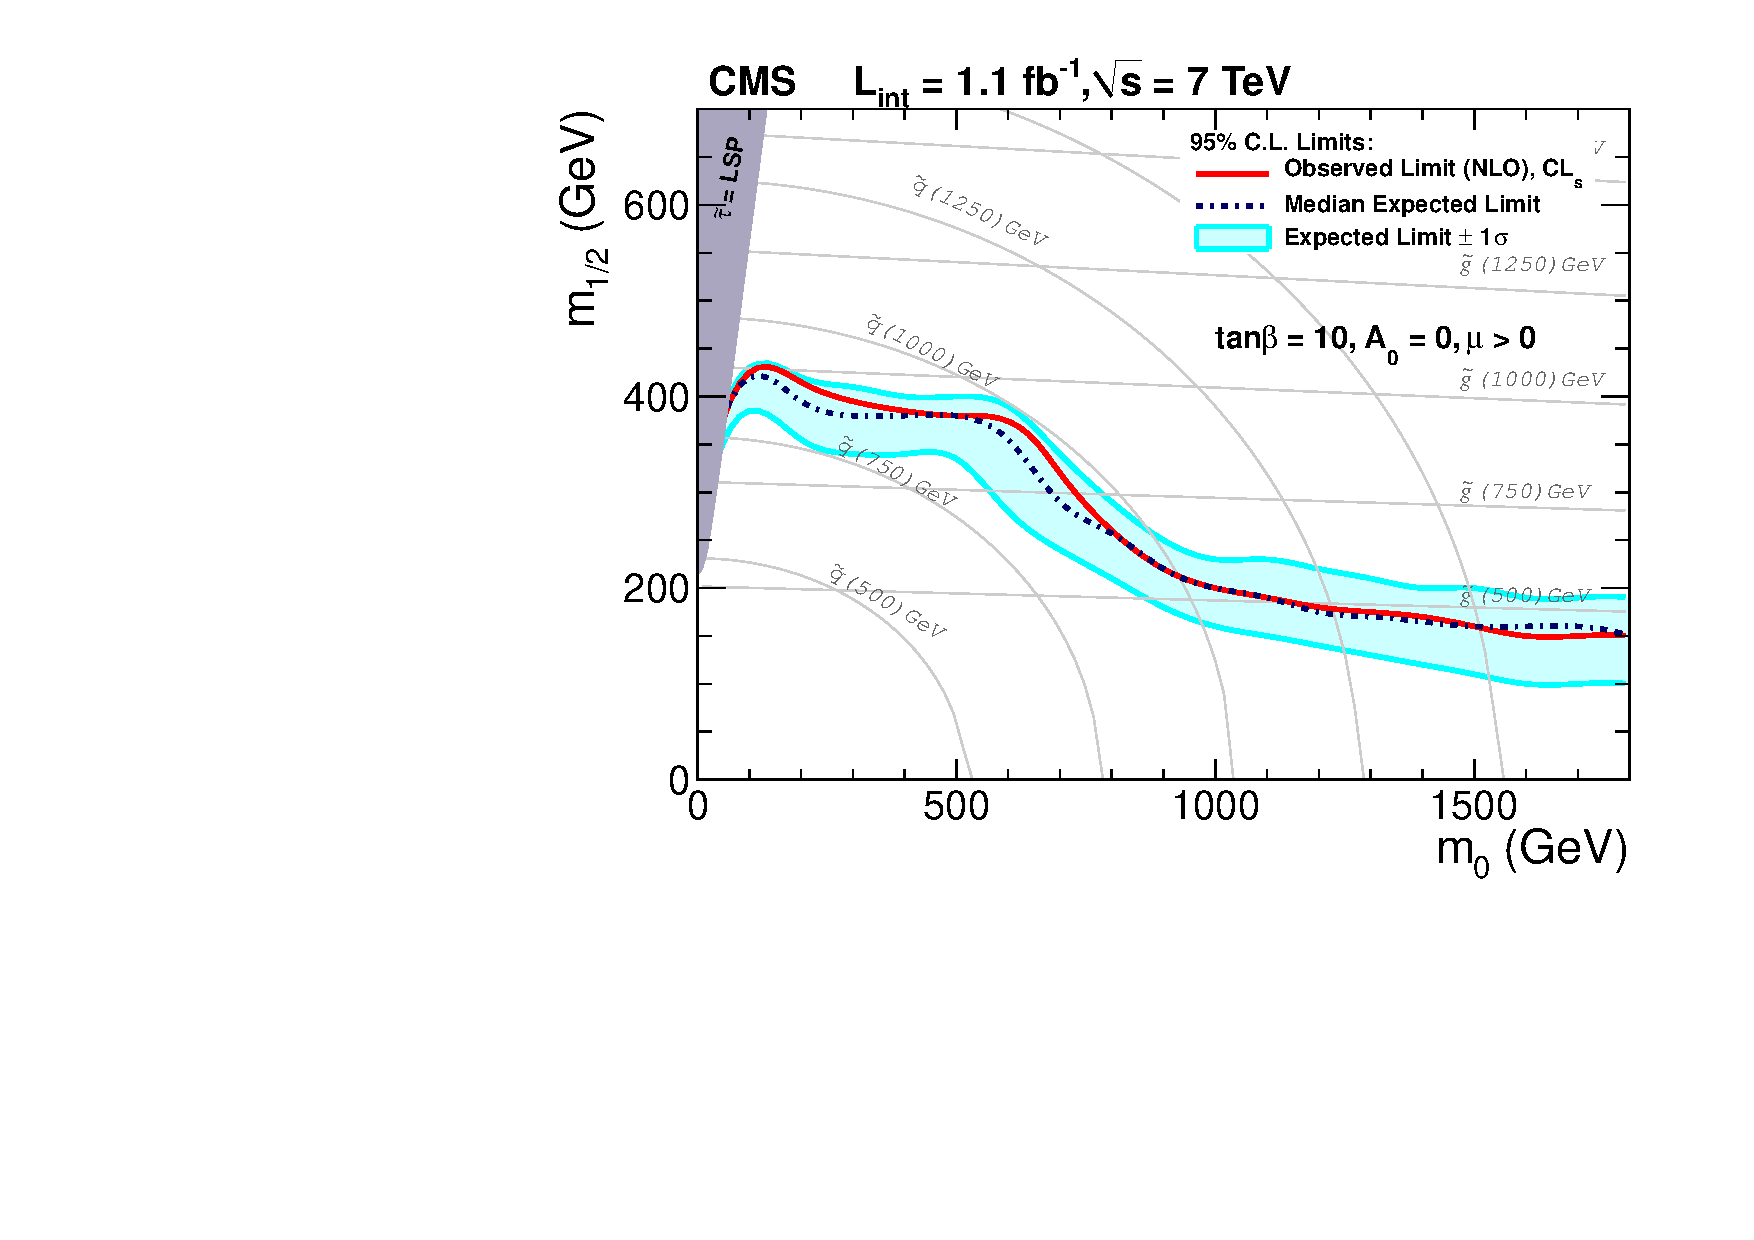
\includegraphics[width=\textwidth]{fig/RA4_ExclusionLimit_tanb10}
\end{figure}